\documentclass{article}
\usepackage[margin=0.5in]{geometry}
\usepackage{pgf}
\usepackage{tikz}
\usetikzlibrary{arrows,automata}
\usepackage[latin1]{inputenc}
\usepackage{caption}

\begin{document}

\begin{figure}
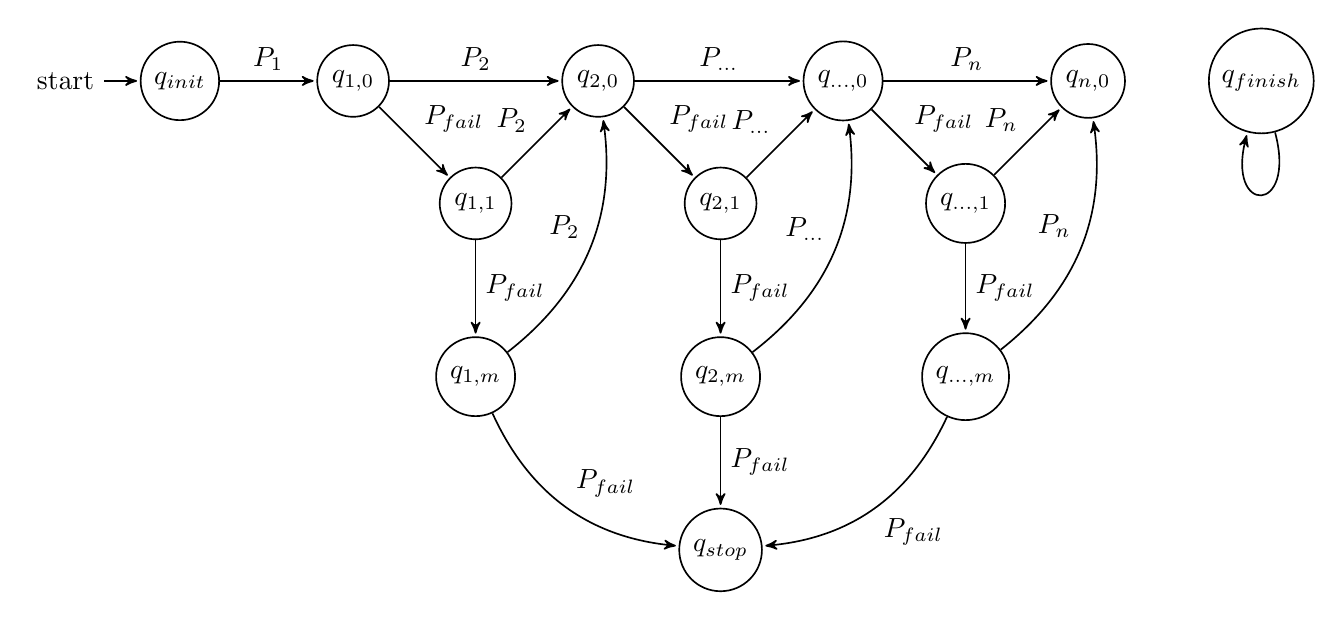
\begin{tikzpicture}[->,>=stealth',shorten >=1pt,auto,node distance=2.2cm,
                    semithick]
  \tikzstyle{every state}=[text=black]

  \node[initial,state] (A)                    {$q_{init}$};
  \node[state]         (B) [right of=A]       {$q_{1,0}$};
  \node[state]         (G) [below right of=B] {$q_{1,1}$};
  \node[state]         (C) [above right of=G] {$q_{2,0}$};
  \node[state]         (H) [below right of=C] {$q_{2,1}$};
  \node[state]         (D) [above right of=H] {$q_{\dots,0}$};
  \node[state]         (I) [below right of=D] {$q_{\dots,1}$};
  \node[state]         (E) [above right of=I] {$q_{n,0}$};
  \node[state]         (F) [right of=E]       {$q_{finish}$};
  

  \node[state]         (K) [below of=G] {$q_{1,m}$};
  \node[state]         (L) [below of=H] {$q_{2,m}$};
  \node[state]         (M) [below of=I] {$q_{\dots,m}$};
  
  \node[state]         (S) [below of=L] {$q_{stop}$};
  
  \path (A) edge              node {$P_{1}$}     (B)
        
        (B) edge              node {$P_{2}$}     (C)
        (B) edge              node {$P_{fail}$}  (G)
        (G) edge              node {$P_{fail}$}  (K)
        (G) edge              node {$P_{2}$}     (C)
        (K) edge [bend right] node {$P_{fail}$}  (S)
        (K) edge [bend right] node {$P_{2}$}     (C)
        
        (C) edge              node {$P_{\dots}$} (D)
        (C) edge              node {$P_{fail}$}  (H)
        (H) edge              node {$P_{fail}$}  (L)
        (H) edge              node {$P_{\dots}$} (D)
        (L) edge              node {$P_{fail}$}  (S)
        (L) edge [bend right] node {$P_{\dots}$} (D)
        
        (D) edge              node {$P_{n}$}     (E)
        (D) edge              node {$P_{fail}$}  (I)
        (I) edge              node {$P_{fail}$}  (M)
        (I) edge              node {$P_{n}$}     (E)
        (M) edge [bend left]  node {$P_{fail}$}  (S)
        (M) edge [bend right] node {$P_{n}$}     (E)
        
        (F) edge [loop below] node {}            (F);
\end{tikzpicture}
\caption{State diagram with probabilities of transitioning into next receiving state.}
\end{figure}

\end{document}
